\subsection{Support Vector Machine}
Support Vector Machines \cite{cortes_support_1995} is a classification algorithm to solve binary-class problems by maximizing margin between data points and linear decision hyperplane. Also, once data is not linearly seperable, new features are generated by nonlinear transformations to convert data linearly seperable in a new feature space. In Figure \ref{fig:svm_margin}, decision boundary is illustrated in linear feature space.

\begin{figure}
	\centering
	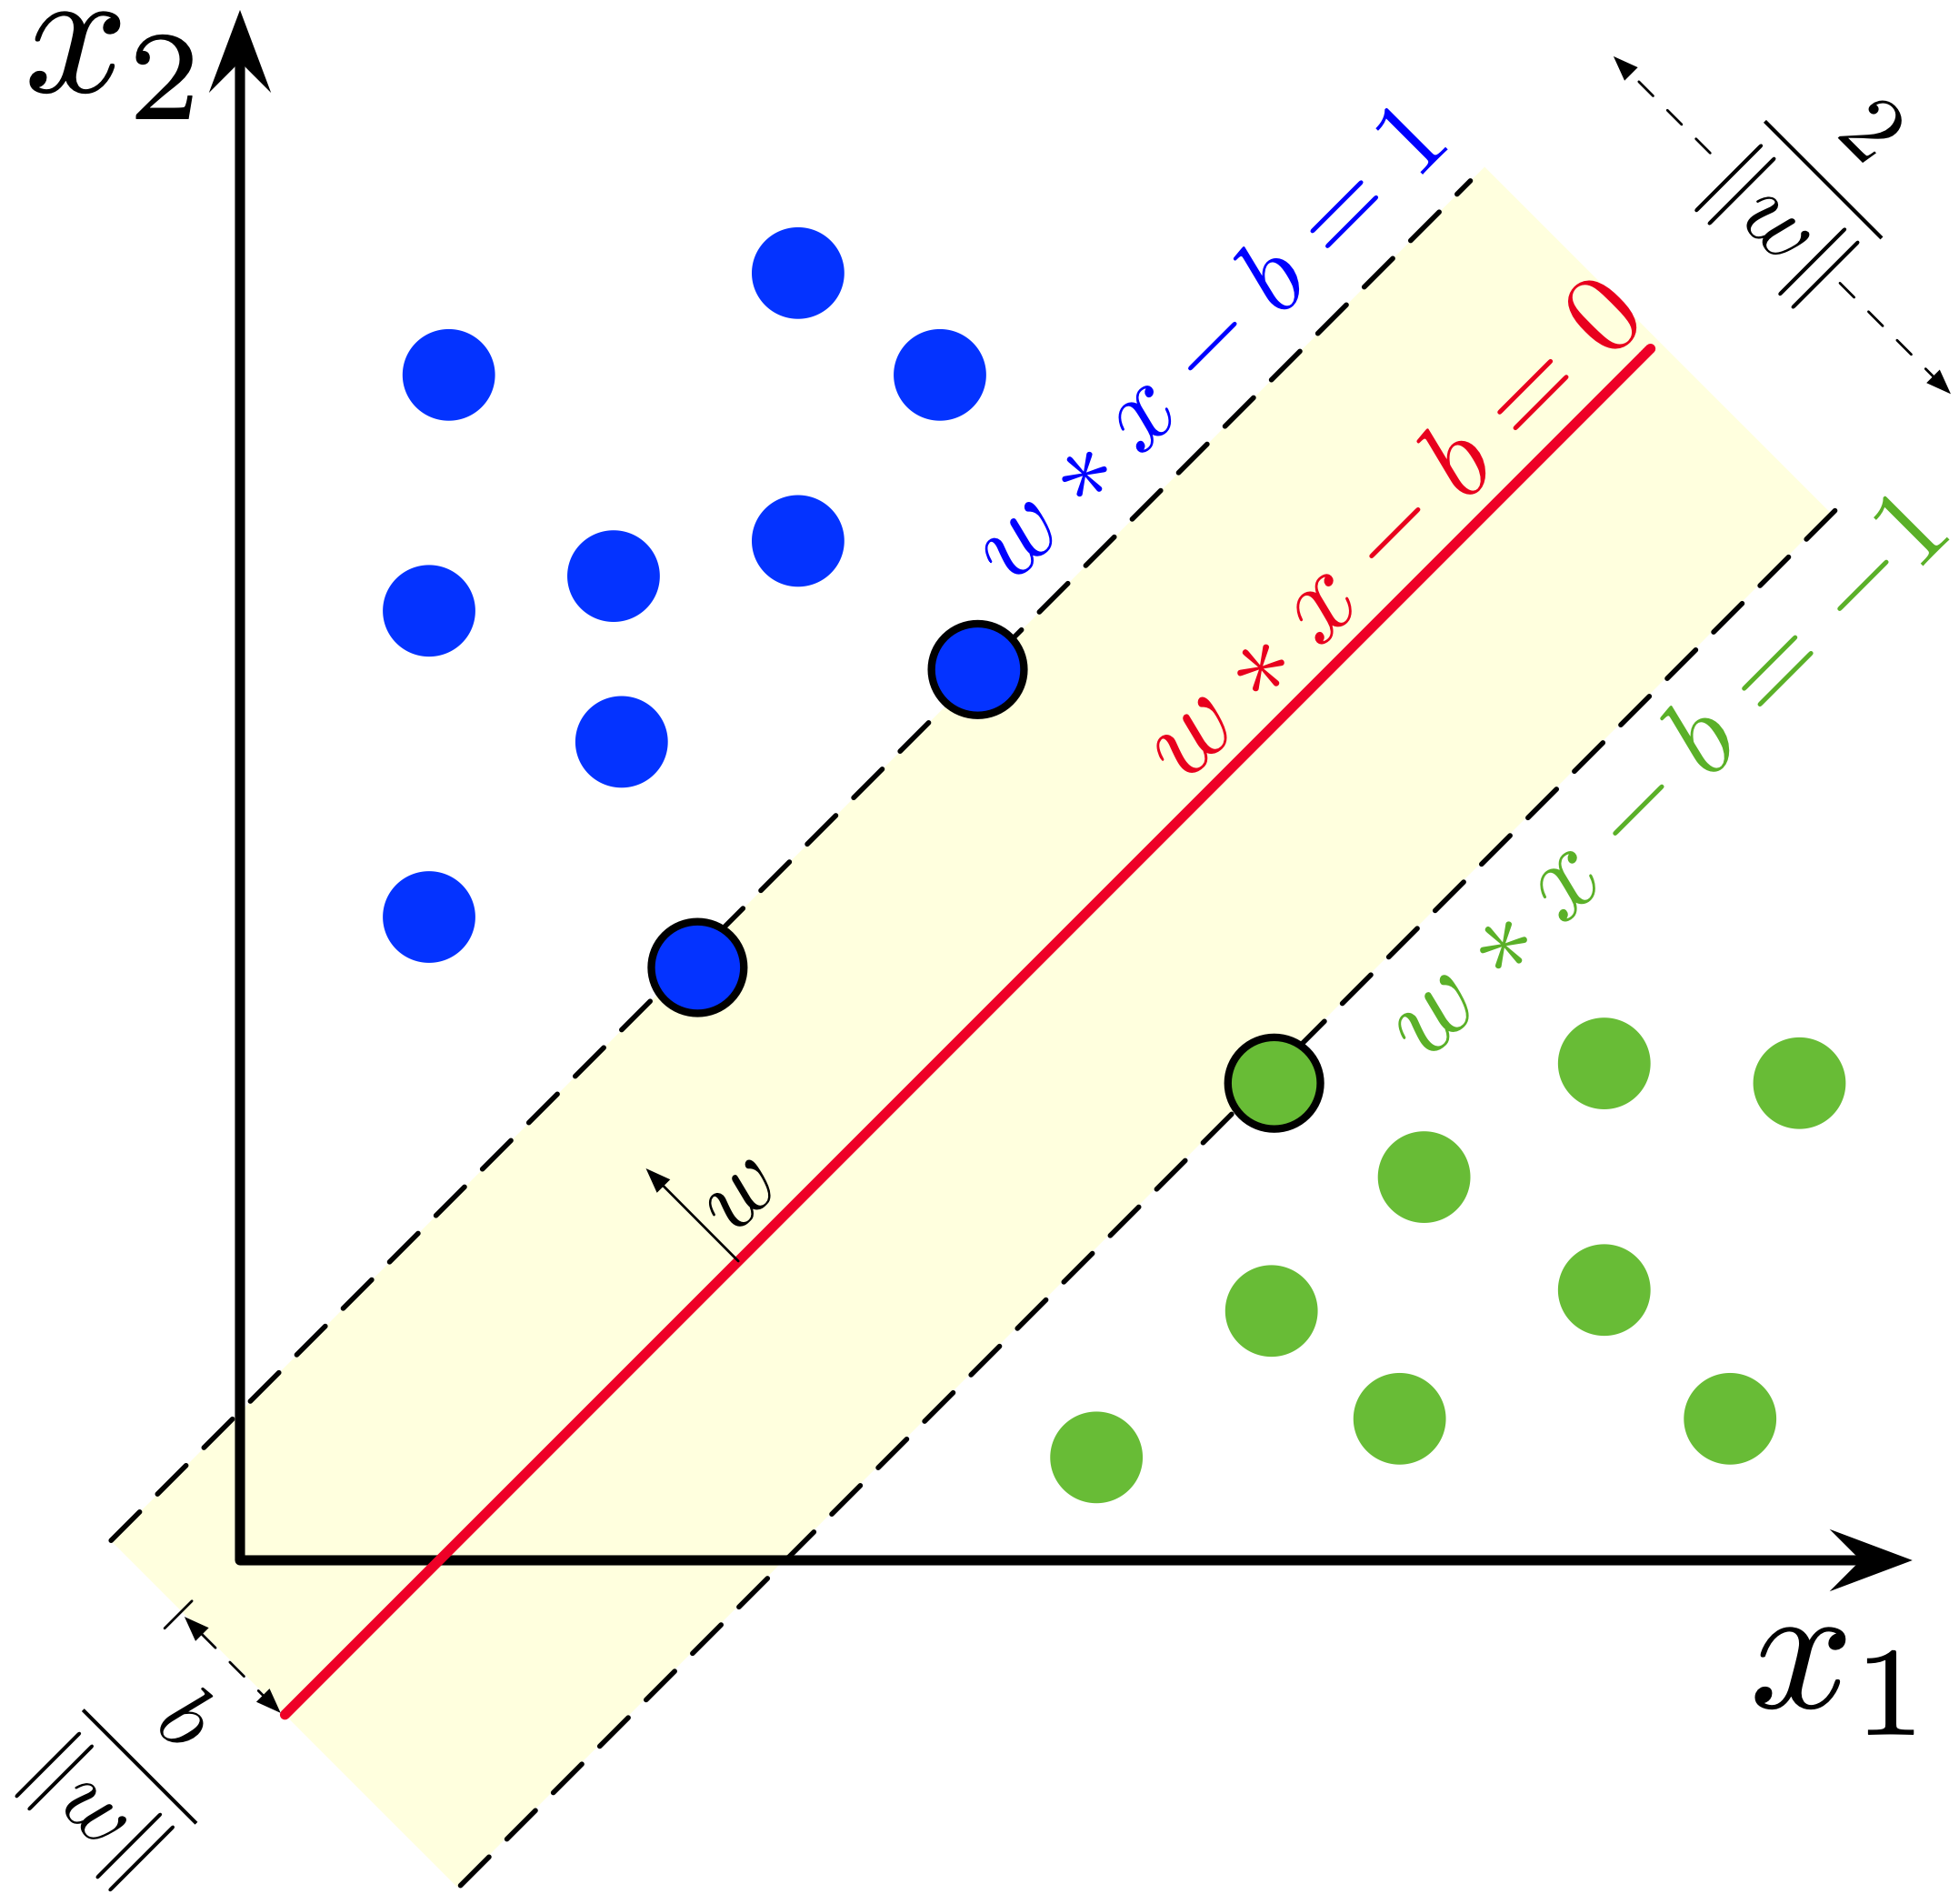
\includegraphics[width=0.75\textwidth]{./figures/ml_theory/SVM_margin.png}
	\caption{SVM Decision Boundary}
	\label{fig:svm_margin}
\end{figure}

For $m$-class classification tasks, $m$ hyperplane is found by SVM algorithm, for each class. In other words, there are $m$ SVM models.

Assume that $N$ data points are given in the following form for binary classification task. Data label is $t_i$ which is either $+1$ or $-1$.
\begin{equation}
(\boldsymbol{x_i}, t_i) \in X \times \{-1,1\}, i=1,2,...,N
\end{equation}

A simple linear classification is finding weight $\boldsymbol{w}$ and bias $b$ for regression of variable $y$ where $y(x)>0$ if $t=+1$ and $y(x)<0$ if $t=-1$.
\begin{equation}
y(x) = \boldsymbol{w}^T \boldsymbol{x} + b
\end{equation}



When the data is linearly seperable, there might be multiple possible solutions for weight and bias. If so, one giving smallest generalization error should be found. The term margin is introduced to maximize generalization.

Margin is minimum distance of any points from the decision boundary. The main idea of Support Vector Machine is to find best seperating hyperplane with largest margin. The perpendicular distance of a point $\boldsymbol{x_i}$ to decision boundary $y(x) = \boldsymbol{w}^T \boldsymbol{x} + b = 0$ is the following.

\begin{equation}
\label{eq:svmmargin}
\frac{t_i y_i}{\| \boldsymbol{w} \|_2} = \frac{t_i (\boldsymbol{w}^T \boldsymbol{x}_i + b)}{\| \boldsymbol{w} \|_2}
\end{equation} 

There is a margin for all data points. However, smallest possible margin is required to be maximized. In equation \ref{eq:svmmargin} numerator should be maximized and denominator should be minimized. Note that scaling parameter $\boldsymbol{w}$ and $b$ does not change distance. Using this freedom, it is possible to assume following inequality for all data points.

\begin{equation}
\label{eq:svm_con1}
t_i y_i = t_i (\boldsymbol{w}^T \boldsymbol{x}_i + b) \geq 1
\end{equation} 

Numerator is no more required to be maximized, because it is constrained to be $1$. Then denominator $||\boldsymbol{w}||_2$ is minimized by quadratic loss. This approach yields the following optimization problem.

\begin{equation}
\label{eq:svm_opt}
\begin{aligned}
&\underset{\boldsymbol{w},b}{\arg\min}&&\frac{1}{2}\boldsymbol{w}^\intercal\boldsymbol{w} \\
&\text{subject to } &&t_i (\boldsymbol{w}^T \boldsymbol{x}_i + b) \geq 1, \; i=1,\ldots,N
\end{aligned}
\end{equation} 

For the optimization problem \ref{eq:svm_opt}, once lagrangian function is constructed with lagrange variables $\boldsymbol{a} \in \mathbb{R}^N$ dual problem seems easier to deal with. Skipping primal problem, setting its derivatives to zero yields the following relations \ref{eq:primaldualrelation}. 
\begin{equation}
\label{eq:primaldualrelation}
\begin{aligned}
&\sum_{i=1}^{N} a_i t_i \boldsymbol{x}_i &= \boldsymbol{w} \\
&\sum_{i=1}^{N} a_i t_i &= 0
\end{aligned}
\end{equation} 

Substituting them generates the dual problem \ref{eq:svm_dualopt1}].

\begin{equation}
\label{eq:svm_dualopt1}
\begin{aligned}
&\underset{\boldsymbol{a}}{\arg\min}&& \sum_{i=1}^{N} a_i - \frac{1}{2}\sum_{i=1}^{N}\sum_{j=1}^{N} a_i a_j t_i t_j \boldsymbol{x_i}^\intercal \boldsymbol{x_j}\\
&\text{subject to } &&\sum_{i=1}^{N} a_i t_i = 0 \\
& && a_i \geq 0, \; i=1,\ldots,N
\end{aligned}
\end{equation} 

The problem is now solvable by quadratic optimization methods.

\subsubsection{Overlapping Class Distributions}
The settings mentioned so far does not let any data points to be misclassified, i.e, there may not be an exact solution. Somehow, we need to let some data points to be misclassified for generalization.
For each data points, slack variables $\xi_i \geq 0$ (which are nonzero for data points exceeding margin) introduced to redefine constraints and cost functions.
Now classification constraints in equation \ref{eq:svm_con1} are redefined in equation \ref{eq:svm_con2}.
\begin{equation}
\label{eq:svm_con2}
t_i y_i = t_i (\boldsymbol{w}^T \boldsymbol{x}_i + b) \geq 1-\xi_i
\end{equation} 
And now, instead of minimizing $||\boldsymbol{w}||_2$ only, the new cost $C\sum_{i=1}^{N} \xi_i + \frac{1}{2}||\boldsymbol{w}||_2$ is minimized by softly penalizing data points exceeding data points, controlled by hyperparameter $C$.
Skipping derivations, only inequality contraint of variable $\boldsymbol{a}$ changed, and problem is in equation \ref{eq:svm_dualopt2} 

\begin{equation}
\label{eq:svm_dualopt2}
\begin{aligned}
&\underset{\boldsymbol{a}}{\arg\min}&& \sum_{i=1}^{N} a_i - \frac{1}{2}\sum_{i=1}^{N}\sum_{j=1}^{N} a_i a_j t_i t_j \boldsymbol{x_i}^\intercal \boldsymbol{x_j}\\
&\text{subject to } &&\sum_{i=1}^{N} a_i t_i = 0 \\
& && C \geq a_i \geq 0, \; i=1,\ldots,N
\end{aligned}
\end{equation} 


\subsubsection{Kernel Trick and Nonlinear SVM}
As stated earlier, SVM is also capable of nonlinear classification, is desired. Instead of using features directly, nonlinear combinations of features can be used to extend feature space using a reasonable transformation $\phi$. In the dual optimization, only $\boldsymbol{x}_i^\intercal\boldsymbol{x}_j$ is enough about data. This is called kernel. However, if nonlinear kernels are defined at first, nonlinear features do not need to be extracted directly. 
Assuming new features are  $\phi(\boldsymbol{x})$, the kernel is simply $k(\boldsymbol{x}_i,\boldsymbol{x}_j)=\phi(\boldsymbol{x}_i)^\intercal\phi(\boldsymbol{x}_j)$

\subsection{Logistic Regression}
Logistic regression is generalization of linear regression idea into discriminative classification. Assume that there are $K$ class and $N$ data points are given with data label $t_i \in [0,1]^6$.

Given a data point $\boldsymbol{x}_i$, its probability to belong to class $c_k$ is evaluated by softmax function \ref{eq:softmaxfun}, after linear transformation.

\begin{equation}
\label{eq:softmaxfun}
p(c_k|\boldsymbol{x}_i) = y_k(\boldsymbol{x}_i) = \frac{\exp(\boldsymbol{w}_k^\intercal\boldsymbol{x}_i+b_k)}{\sum_{j=1}^{K} \exp(\boldsymbol{w}_j^\intercal\boldsymbol{x}_i+b_j)}
\end{equation} 

Then parameters $\boldsymbol{w}_j, \; j=1,\ldots,K$ are learned by optimizing cross entropy loss \ref{eq:crossentropy} using any algorithm.

\begin{equation}
\label{eq:crossentropy}
L(\boldsymbol{w}_1,\ldots,\boldsymbol{w}_K,b_1,\ldots,b_K) = -\sum_{i=1}^{N}\sum_{j=1}^{K} t_{nk} \log(y_{nk})
\end{equation} 

\subsubsection{Regularized Logistic Regression}

The only difference is definition of loss function. New loss function is \ref{eq:regcrossentropy} with a new hyperparameter $C$ controlling regularization.

\begin{equation}
\label{eq:regcrossentropy}
L(\boldsymbol{w}_1,\ldots,\boldsymbol{w}_K,b_1,\ldots,b_K) = -\frac{C}{N}\sum_{i=1}^{N}\sum_{j=1}^{K} t_{nk} \log(y_{nk}) + \frac{1}{2}\sum_{j=1}^{K} ||\boldsymbol{w}_j||^2
\end{equation} 

\subsubsection{Nonlinear Logistic Regression}

Unlike SVM, logistic regression does not include nonlinearity. However, instead of using features directly, nonlinear transformation may be applied before logistic classifier. Most well-known method is neural networks, which is a method of generalized nonlinear regression. The benefit of logistic regression arises here. It allows neural network and itself to be trainable at the same time, where SVMs require untrainable kernel functions.

